\chapter{Opis struktury projektu}
Diagram klas reprezentuje schemat powiązań pomiędzy klasami i encjami w bazie danych. Pola, które znajdują się w tabelach, są właściwościami w klasach i zawierać będą wartości, które będą zapisane w bazie. Na łączeniach pomiędzy tabelami widać rodzaj relacji.
\section{Diagram klas}
\begin{figure}[!ht]
	\centering
		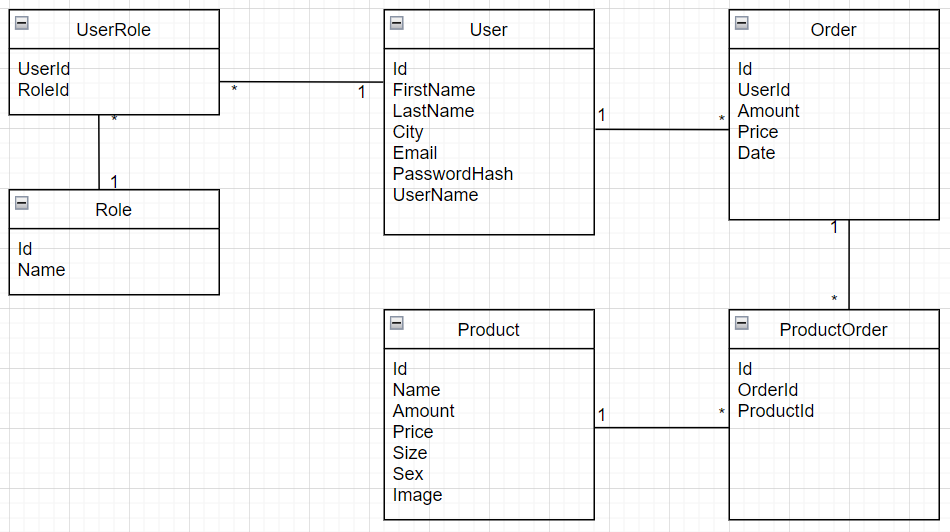
\includegraphics[width=15cm]{diagram.png}
	\caption{\footnotesize Diagram klas programu Sklep}
	\label{fig:plotend}
\end{figure}

Powyższy diagram przedstawia klasy, które reprezentują dane użytkownika, produktów oraz zamówień. Klasy odpowiadające na dane klienta oraz role w systemie zostaną wygenerowane przez bibliotekę Identity, która służy do autoryzacji i autentykacji użytkowników. Udostępnia ona również gotowe mechanizmy logowania, rejestracji i wiele innych. Użytkownik połączony jest z rolą w relacji wiele do wielu, dlatego też istnieje klasa łącząca UserRole.\newline

W takiej samej relacji znajdują się klasa Product oraz Order. Jeden produkt może znajdować się w wielu zamówieniach i tak samo jedno zamówienie może zawierać wiele produktów, przez co w tym przypadku również zastosowano powiązanie poprzez klasę łączącą. Użytkownik może mieć wiele zamówień w sklepie, a jedno zamówienie przypisane jest tylko do jednego klienta, przez co połączony jest w relacji jeden do wielu.\newline

Klasa użytkownika zawiera podstawowe informacje o kliencie, poprzez które będzie można go zweryfikować. Produkt zawiera informacje takie jak nazwa, ilość sztuk dostępna w sklepie, cena za sztukę, rozmiar, płeć, oraz obrazek, który w formie ascii artu będzie przedstawiał dany artykuł na konsoli. Natomiast tabela Order przechywać będzie dane o zamówieniu takie jak kto i kiedy złozył zamówienie ilość produktów oraz całkowita kwota zamówienia.